\paragraph{\trAcyclic{}性。}\label{sub:acyclicity}
[131, Lemma 2.32] 证明中的那些代数论证，再加上 [131, Chapter 3] 中的那些几何论证，证明了 \eqref{eq:auxiliary-complex-differential} 中定义的\trComplex{} $D$ 是\trAcyclic{}的；鉴于\cref{thm:quasi-representative-criterion}(iii)，这一点对我们十分重要。严格说来，[131] 只是在下列若干附加技术条件下才建立了\trAcyclic{}性：
(i) $Q$、$L_0$、$L_2$ 处于\trGeneralPosition{}。诸对 $(Q,L_0)$、$(L_0,L_2)$ 与 $(Q,L_2)$ 的\trFloerDatum{}应当具有零\trHamilton{}项。此外，在交点处，诸\trActionFunctional（\eqref{eq:perturbed-action}）的取值还须满足一个条件：即，$x_0\in\scr{C}(Q,L_2)$ 时的诸数 $A(x_0)$，以及 $(x_1,x_2)\in\scr{C}(Q,L_0)\times\scr{C}(L_0,L_2)$ 时的诸数 $A(x_1)+A(x_2)$，必须全都两两不同。
(ii) 需要能够把\trFrame{}$L_0=V\cong S^n$ 扩张成\trCotangent{}球丛的一个\trSymplectic\trEmbedding{}$B_s^*S^n\to\mathrm{int}(M)$（对某个 $s>0$），使得 $\theta_M$ 的\trPullback{}是 $T^*S^n$ 上的标准 $1$-形式。此外，在这个\trTubularNeighborhood{}中，$Q$ 与 $L_2$ 都应当是若干\trCotangentFibre{}之并。
(iii) $L_1=\tau_V^{-1}(L_2)$，其中\trDehnTwist{}是利用先前选定的那个\trTubularNeighborhood{}来定义的。决定扭转速度的函数 $b$（\eqref{eq:dehn-twist-function}）必须满足某些条件；这些条件既依赖于 (i) 中诸作用值之间的极小差，也依赖于点 $x_1,x_2$ 之间关于 $V$ 上\trSphere\trMetric{}的极小距离。
(iv) 诸对 $(L_0,L_1)$ 与 $(Q,L_1)$ 的\trFloerDatum{}应当具有零\trHamilton{}项；同样，三元组 $(Q,L_0,L_1)$ 的\trPerturbationDatum{}应当满足 $K=0$。
(v) 最后，进入 $(d,l)$ 定义之中的那些辅助几何数据（\trLefschetzFibration、\trLagrange\trBoundaryCondition、\trRelative\trPerturbationDatum）必须以受到精确控制的方式来选取。
作为一个初步的观察，如果愿意作如下改动，那么所有这些条件都可以被满足：对诸 $L_k$ 作\trLagrange\trIsotopy；把 $\theta_M$ 换成 $\theta_M+dh$（$h$ 是某个\trSupport{}落在 $\mathrm{int}(M)$ 中的函数）；以及更改用来定义\trFukayaCategory{}的\trFloerDatum{}与\trPerturbationDatum。由于这些改动没有一个会在\trCohomology{}层面上影响\trObject{}的\trIsomorphism{}类（无论是在\trFukayaCategory{}中，还是在其\trAinfty-模\trCategory{}中），我们可以应用\cref{thm:quasi-representative-criterion}(iii) 而直接得出 $\scr{T}_{Y_0}(\scr{Y}_1)\cong\scr{Y}_2$。这对大多数用途而言已经足够好，但还不能完全令人满意，因此我们将借助\cref{sub:additional-remarks-17f}中的结果着手进行更细致的分析。首先，(v) 显然是不必要的，因为正如我们在\eqref{eq:chain-complex-isomorphism-17f}中所看到的，$D$ 的\trIsomorphism{}类不依赖于那些选取。
类似地，\eqref{eq:chain-map-alpha-beta} 表明了与 $L_1$ 的无关性，这使我们能够去掉 (iii)；由于 (ii) 中那个\trTubularNeighborhood{}只是被用来定义 $L_1=\tau_V^{-1}(L_2)$ 的，它也随之成为多余；此外，换成\trIsotopy{}的 $\tilde{L}_1$ 还意味着与该\trSubmanifold{}相关联的\trFloerDatum{}可以完全自由地选取，而这在先前是受 (iv) 约束的。一个与 $L_1$ 的情形相平行的论证表明，我们可以把 $L_2$ 在其\trIsotopy{}类之内移动，而不影响 $D$ 的\trQuasiisomorphism{}类；最后，正如\cref{thm:quasi-representative-criterion}(iii) 中已经提到过的，$(d,l)$ 经由 \eqref{eq:xi-psi} 与 $(c,k)$ 相联系这一事实意味着：\eqref{eq:auxiliary-complex-differential} 对某个 $Q$ 的\trAcyclic{}性，蕴含它对所有\trIsotopy{}的 $\tilde{Q}$ 也同样成立。合在一起，这就使得 (i) 与 (iv) 的剩余部分都成为不必要的了。于是我们已经证明：\emph{来自 \eqref{eq:auxiliary-complex-differential} 的\trComplex{} $D$ 是\trAcyclic{}的，对一切 $(L_0,L_1,L_2,Q)$ 皆然，并且与定义 $(d,l)$ 时所作的选取无关。}用\cref{thm:quasi-representative-criterion}的话来说，这意味着由 $(c,k)$ 定义的\trMorphism{}$\scr{T}_{Y_0}(\scr{Y}_1)\to\scr{Y}_2$ 总是一个\trIsomorphism。
\begin{remark}\label{thm:additional-data-gpq}
为了给这场讨论收尾，我们想大致勾画一下如何造出满足\cref{thm:third-morphism-realization}中诸条件的附加代数数据 $(g,p,q)$。在\trCohomology{}层面上，$[g]$ 与延续\trIsomorphism
$HF^{\mathrm{pr}}(L_0,L_2)\to HF^{\mathrm{pr}}(L_0,\tau_V(L_1))\cong HF^{\mathrm{pr}}(L_0,L_1)$ 是\trPoincare{}对偶的。我们可以用一个技巧来简化任务：这样来选取 $(L_2,L_0)$ 的\trFloerDatum，使得其上链群自然地对偶于 $(L_0,L_1)$ 的那个。如果 $L_2$ 等于 $\tau_V(L_1)$，那么如何做到这一点是显而易见的：只需取 $(L_0,L_1)$ 的\trFloerDatum{}$(H,J)$，把它换成 $(-H(-t),J(-t))$，然后再对它施加 $\tau_V$。一般地，$L_2$ 只是\trIsotopy{}于 $\tau_V(L_1)$，但可以把该\trIsotopy{}纳入上面定义的那个\trFloerDatum{}的一个修改版本之中，从而将其考虑在内。现在，取 $g$ 为恒等映射 $CF^{\mathrm{pr}}(L_2,L_0)^{\vee}\to CF^{\mathrm{pr}}(L_0,L_1)$ 的对偶。记住了这一点，其余各项及其所需性质便可写作
\begin{equation}\label{eq:gpq-datum}
\boxed{\begin{aligned}
&p\colon CF^{\mathrm{pr}}(L_2,L_0)\longrightarrow CF^{\mathrm{pr}}(L_1,L_0),\\
&q\colon CF^{\mathrm{pr}}(L_2,L_0)\otimes CF^{\mathrm{pr}}(L_0,L_1)\longrightarrow CF^{\mathrm{pr}}(L_0,L_0),\\
&\mu^1(p(\cdot))+p(\mu^1(\cdot))+\mu^2(\cdot,c)=0,\\
&\mu^1(q(\cdot,\cdot))+q(\mu^1(\cdot),\cdot)+q(\cdot,\mu^1(\cdot))\\
&\quad+\mu^3(\cdot,c,\cdot)+\mu^2(\cdot,k(\cdot))+\mu^2(p(\cdot),\cdot)\\
&\quad+e\langle\cdot,\cdot\rangle=0;
\end{aligned}}
\end{equation}
其中最后一行里的 $\langle\cdot,\cdot\rangle$ 是对偶\trPairing，而 $e\in CF^{\mathrm{pr}}(L_0,L_0)$ 是\trCohomology{}恒等元的一个代表。从其中第一个方程清楚可见，应当如何通过改造上面 $k$ 的定义来构造 $p$。至于 $q$，我们考虑 $\scr{R}^{3,1}$ 上的一个双参数\trFamily，如 \cref{fig:hexagon-degenerations} 中那样，但现在取 $Q=L_0$。来自边界边 (i)、(ii) 与 (vi) 的贡献产生了 \eqref{eq:gpq-datum} 倒数第二行中的那些项，而来自 (iii) 与 (v) 的那些则消没。这就只剩下 (iv) 这个最后也最有意思的情形了。相关的几何设置由两个\trLefschetzFibration{}组成，二者在边界\trMarkedPoint{}之上的\trFiber{}之间带有一个等同关系（\cref{fig:identified-fibrations}）。左边的那个块记作 $E^e\to S^e$，其\trMarkedPoint{}的位置是可变的，因此我们得到一个带额外参数的\trEvaluationMap。设 $(L_0,L_0)$ 的\trFloerDatum{}取得使\trHamilton{}量是 $L_0=S^n$ 上的一个标准\trMorseFunction，从而 $CF^{\mathrm{pr}}(L_0,L_0)$ 有两个\trGenerator{}$e=y_0$ 与 $y_n$。于是，\trModuliSpace{}$\scr{M}_{E^e/S^e}(y_0)$ 与 $\scr{M}_{E^e/S^e}(y_n)$ 的维数分别为 $n-1$ 与 $2n-1$。取其中第一个空间，并考虑\trParametrization{}的\trEvaluationMap，此时我们利用\trParallelTransport{}把 $\partial S^e$ 上任一点处的\trLagrange\trBoundaryCondition{}与 $L_0$ 等同起来：
\begin{equation*}
\mathrm{ev}\colon\RR\times\scr{M}_{E^e/S^e}(y_0)\longrightarrow L_0.
\end{equation*}
可以证明，$\mathrm{ev}$ 在 $L_0\setminus\{y_0,\tau_V(y_0)\}$ 上是奇\trDegree{}的（缺失的两个点对应于 $z$ 趋于无穷的极限）。证明的办法是先化归到闭\trDisk{}的情形，再化归到标准局部模型；与 [131, Remark 2.17 (iii)] 相比较。一旦有了这一点，就容易看出 (iv) 的贡献确实正是 $e\langle\cdot,\cdot\rangle$。
\begin{figure}[htbp]
\centering
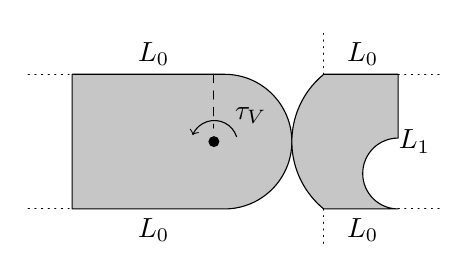
\begin{tikzpicture}[line cap=round,line join=round,scale=0.9]
\draw[fill=gray!45] (0,0) -- (2.15,0) arc[start angle=-90,end angle=90,radius=0.95] -- (0,1.9) -- cycle;
\draw[dotted] (-0.62,1.9) -- (0,1.9);
\draw[dotted] (-0.62,0) -- (0,0);
\fill (2.0,0.95) circle (2.2pt);
\draw[dashed] (2.0,1.9) -- (2.0,1.14);
\draw[->] (2.32,1.02) arc[start angle=18,end angle=158,radius=0.33];
\node at (2.52,1.32) {$\tau_V$};
\node at (1.15,2.18) {$L_0$};
\node at (1.15,-0.3) {$L_0$};
\draw[fill=gray!45]
  (4.6,1.45) -- (4.6,1.9) -- (3.55,1.9)
  arc[start angle=129.3,end angle=230.7,radius=1.228]
  -- (3.55,0) -- (4.6,0)
  arc[start angle=270,end angle=90,radius=0.5] -- (4.6,1.45) -- cycle;
\draw[dotted] (4.6,1.9) -- (5.25,1.9);
\draw[dotted] (4.6,0) -- (5.25,0);
\draw[dotted] (3.55,1.9) -- (3.55,2.55);
\draw[dotted] (3.55,0) -- (3.55,-0.55);
\node at (4.83,0.95) {$L_1$};
\node at (4.1,2.18) {$L_0$};
\node at (4.1,-0.3) {$L_0$};
\end{tikzpicture}
\caption{}\label{fig:identified-fibrations}
\end{figure}
\end{remark}
